\section{Analysis of MRI images dataset}
\subsubsection*{MRI and the NIFTI file format}
\subsubsection*{MRI and the NIFTI file format}
Describe images and dataset: During this activity, a description of the dataset will be generated with a view of the quality of the dataset for the aim of the project and any findings which could result.
\subsubsection*{Loading images}
Extract 2D images: Load 3D images and extract 2D slices from the original dataset, which will be depicted with code.

The NIFTI protocol stores the 3D 

After loading NIFTI images with the nibabel library \dots

\begin{figure}[ht]
    \centering
    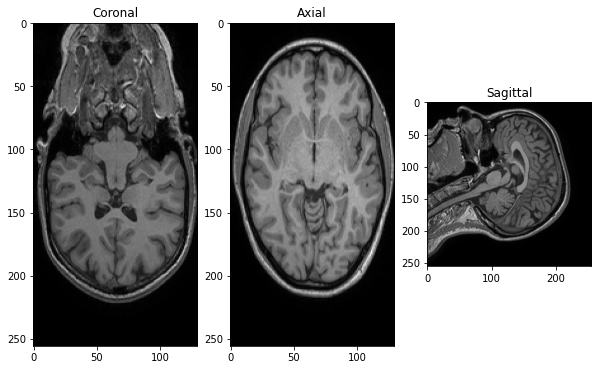
\includegraphics[width = 10cm, height = 6cm]{images/3-axis.png}
    \caption[]{Coronal, Axial and Sagittal images}
    \label{fig:3-axis}
\end{figure}

Images are loaded in the following shape:

\begin{itemize}
    \item 256 Coronal or trasversal plane 
    \item 256 Axial or horizontal plane
    \item 130 Sagittal
\end{itemize}

\subsubsection*{Deciding what slices to use}

Looking at the three different slices in Figure \ref{fig:3-axis}, it is obvious that images have not been processed to show only the brain. The aim of the project is to create artificial brain images, not head images. A model that would learn head images would require much more time and resources than for learning just the brain (which is not a an easy task at all either).

While observing the BraTS \cite{brats} challenge dataset and project description, the skull stripping concept arise. Before publishing the dataset, slices are processed to remove anything that does not pertain to brain. 

This project cannot afford such implementation within the project scope. So, when deciding what slices to use, it became the only decision factor. It happened to be that the rest of considerations where just debatable. 

In conclusion, the noise that bones, eyes and the rest of the items visible in coronal and sagittal axis look very high compared to the axial slices in where, properly selected, slices will only show a surrounding skull bone.

Once that the axial slices were chosen, a sample of brain scans were visually analyzed to find a range of slices that could be used.

The range must exclude as much non-brain pixels as possible while and that happens using the range that goes from above eyes to the top.

\begin{figure}[ht]
    \centering
    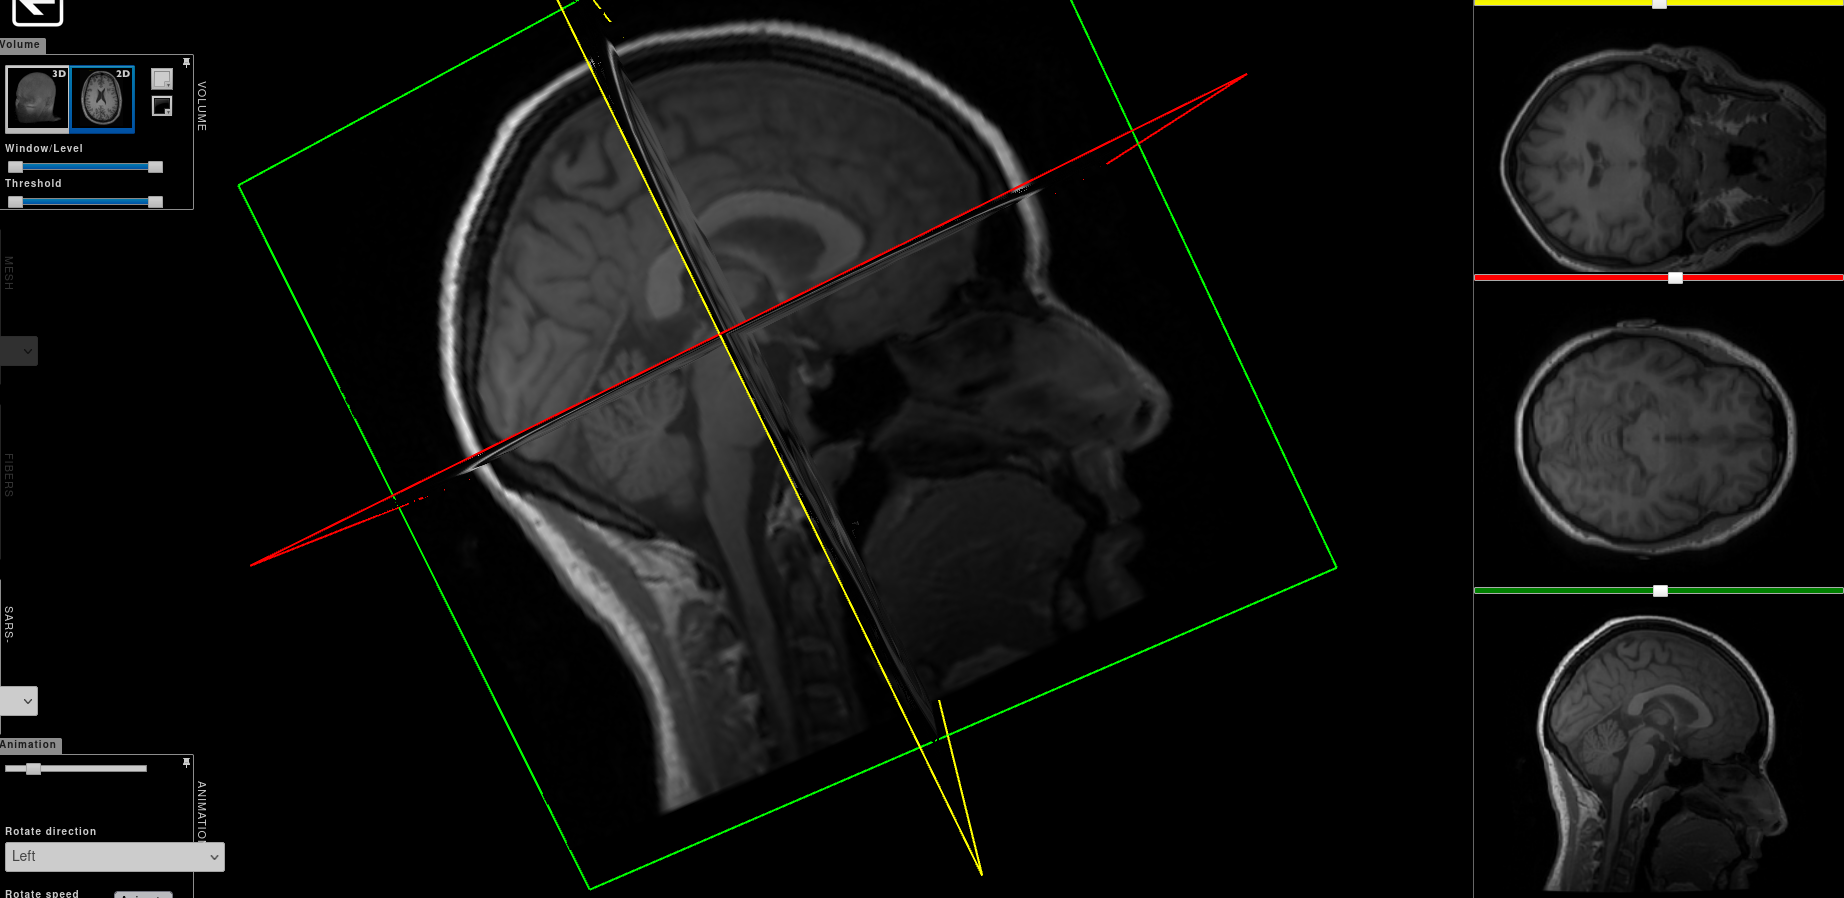
\includegraphics[width = 10cm, height = 6cm]{images/nifti-slice160.png}
    \caption[]{In red, slice 160 as bottom delimiter}
    \label{fig:slice160}
\end{figure}

Also, the slices closer to the top were also discarded to avoid higher heterogeneity on brain images and sizes.

\begin{figure}[ht]
    \centering
    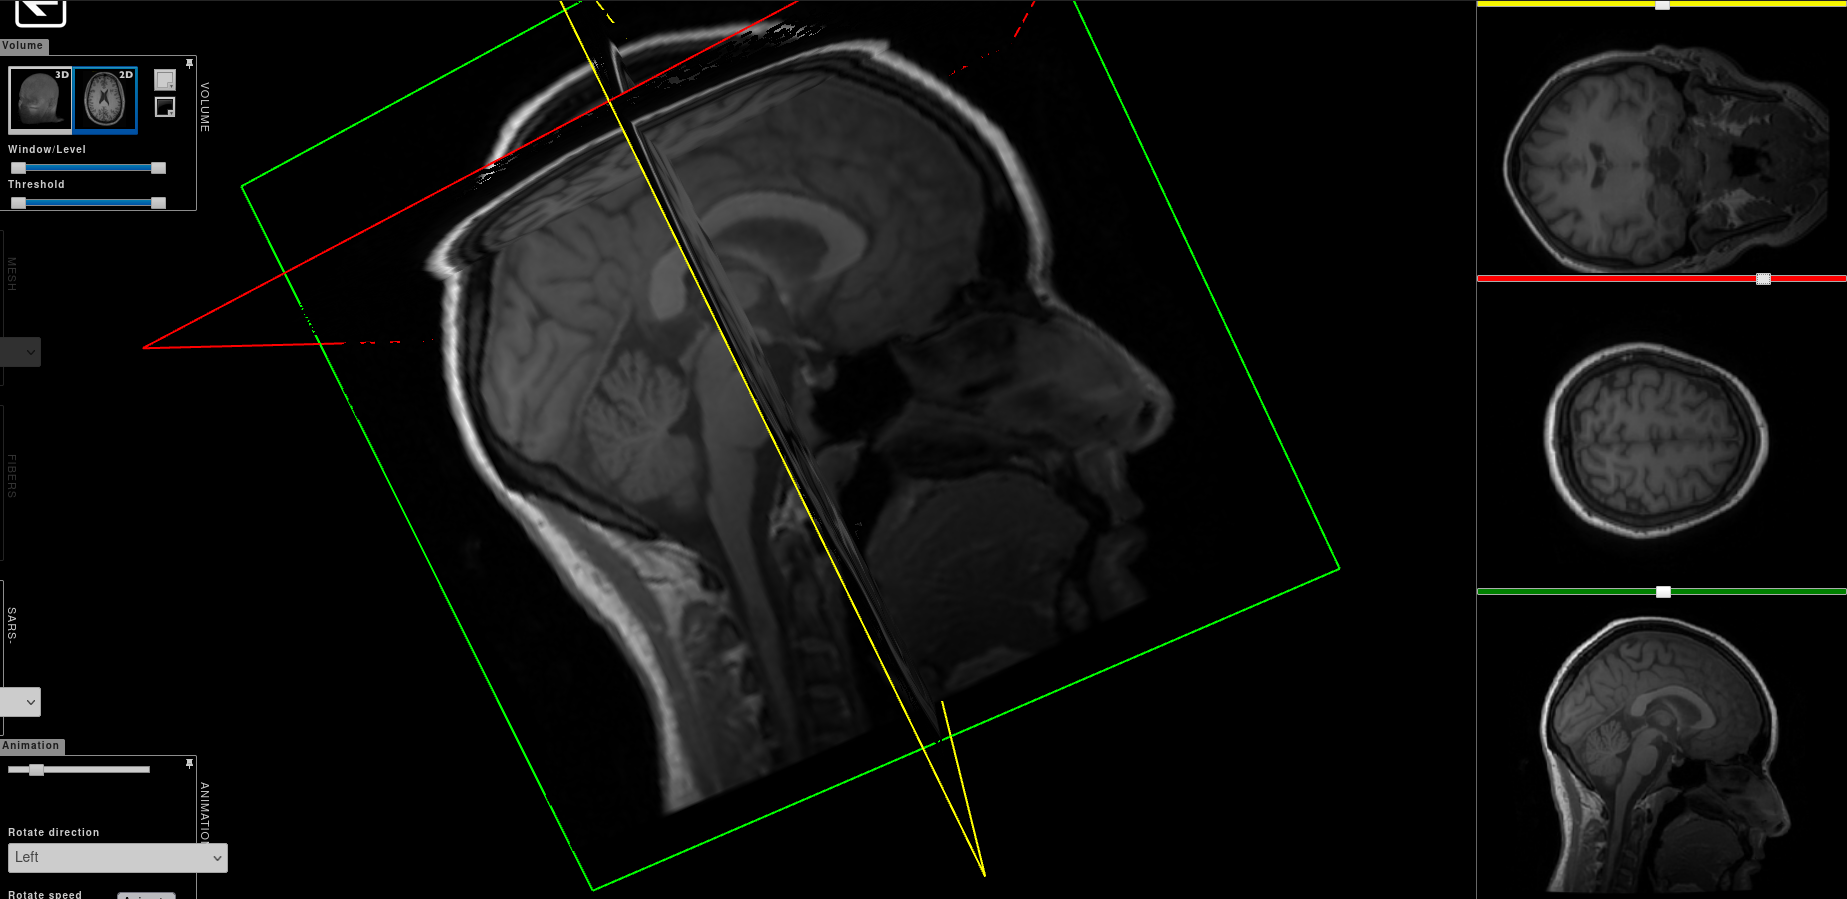
\includegraphics[width = 10cm, height = 6cm]{images/nifti-slice190.png}
    \caption[]{In red, slice 190 as top delimiter}
    \label{fig:slice190}
\end{figure}

It can be interpreted that 3D images are in use since 30 slices of each brain are used which constitue a 3D section of a brain. But, similarly, it could be interpreted that each and every slice of those 30 could happen to be data augmentation or different people with very similar brains.

\subsubsection*{Data Pre-processing and Data Augmentation}

Different pre-processing and data augmentation techniques were briefly evaluated to decide wheter they would improve the model's results. The following table shows the decisions made on each evaluated technique:

\begin{table}
    \centering
    \begin{tabular}{p{3cm}|p{2cm}|p{6cm}}
        \hline
        Technique & Decision & Justification \\
        \hline
        Gray scale & Approved & Applying gray scale to scans seems a natural choice and is usually applied on image processing \\
        Rescaling & Approved & Rescaling \acrshort{rgb} values from 0-256 to 0-1 that can be better handled by the model  \\
        Pixel & Approved & Down-pixeling images from 256 to 128 which requires much less resources and wouldn't lose much quality \\
        Shear Intensity & Declined & Slanting images would distort the latent space leading to create distorted artificial images \\
        Shifts and Rotation & Declined & Similar to shear intensity shifting
            images is seen as a method not accurate for MRI processing as NIFT 
            images will not appear shifted in any prediction phase \\
        Add Noise & Declined & Adding noise is interesting for improving results and key to allow model transfering to other datasets obtained with different scanners and their settings or image quality. It was declined due to time constraints. \\
        \hline
    \end{tabular}
\end{table}

\subsubsection*{Storing data}

In order to isolate image loading from model training into different steps, selected 2D images are stored in \acrshort{png} format after being pre-processed. 

The images are stored in 2 different directories spliting the dataset into 90\% for training and 10\% for test subsets resulting in 16.268 and 1.162 images respectively.



It was concluded that some of them could badly interfere into the latent space representation. For example,  
Due to time constraint other data augmentation techniques were not implemented.

\begin{enumerate}
    \item Gain knowledge on MRI and the NIFTI file format: This activity consists of reading papers and documents to gain sufficient knowledge to execute the project. There is no need to become an expert on the matter but understanding how those files are and how to process them.
    \item 
    \item 
    \item Pre-processing images: Decide which transformations on the 2D images would help the project like pixel changes or applying gray-scale transformations.
\end{enumerate}

